Batteries may compromise the viability of sensor nodes in various ways. Batteries are bulky, short-lived, hazardous, and expensive. To ameliorate the battery problem, researchers have been investigating different alternatives to extend lifetime and reduce costs and form factor.  
The reduction in power consumption of recent microcontrollers (MCUs) and the advances in energy-harvesting (EH) circuitry have enabled the emergence of battery-free EH sensors. 
These sensors elide the constraints of batteries and extract power from ambient energy sources such as sunlight and RF emissions. 

Ambient energy sources provide perpetual power. However, ambient power is usually too weak to directly power a sensor node~\cite{liu2013ambient}.  Therefore, an EH  node first buffers the harvested energy until a usable amount has been accumulated; then it operates, for a short period of time, until the buffered energy has been exhausted~\cite{lucia2017intermittent}.  Consequently, battery-less EH sensors operate intermittently (Figure~\ref{fig:intermittent_opertaion}).

Intermittent power introduces a set of new challenges that are under ongoing investigation.
For example, \cite{lucia2017intermittent,ransford2011mementos,dino,colin2016chain,balsamo2014hibernus,rodriguez2018restop} studied the intermittent computation problem, which is concerned with the preservation of application progress and data consistency under frequent power failures; the authors of \cite{hester2017timely} investigated the timely operation challenge, which is concerned with data freshness after a power interrupt; 
and \cite{yildirim2018ink} introduced event-driven execution for the intermittent domain, which deals with input and output operations under arbitrarily-timed power loss.

Despite these notable advances, intermittently-powered sensors suffer from a new fundamental shortcoming: \textit{the intermittent availability of the system}. Being frequently off charging compromises the value of these devices. For example, a sensor that has a low probability (e.g., 10\%~\cite{coala}) to be available (on) when an event of interest occurs has no value. 
Overcoming the intermittent availability challenge without changing the size of the device or re-including batteries requires a novel approach that explores new design dimensions. 
%
\begin{figure}[b]
	\centering
		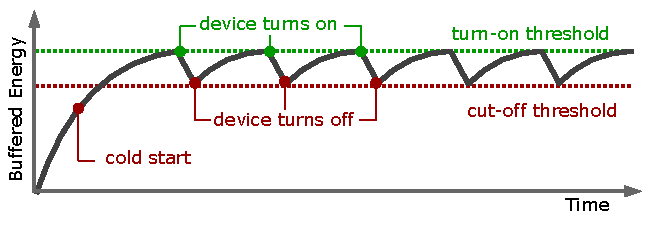
\includegraphics[width=\columnwidth]{figures/intermittent_operation}
		\caption{Harvested-energy profile. Ambient power is weak; therefore, it is usually buffered. The buffered energy is then consumed to operate the device. The operation period is often short as power consumption is much higher than the energy harvesting rate.}
		\label{fig:intermittent_opertaion}
\end{figure} 
%
\subsection{Vision and Application}
%
\begin{figure}[t]
	\centering
	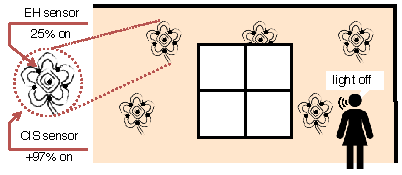
\includegraphics[width=\columnwidth]{figures/smart_fabric}
	\caption{A \fullcis (\cis) is a group of intermittently-powered nodes that sense continuously despite the intermittent power supply. \cis exploits the inherent randomization of energy harvesting systems, if available, and introduces artificial randomization, when needed, to preserve continuous sensing.}
	\label{fig:smart_fabric}
\end{figure}
%
Miniaturized sensors are non-intrusive devices. Therefore,
they can be embedded in locations that are not suited for the others (enabling
new applications). Miniaturizing sensors, however, introduces the significant
challenge of powering them.
%
On the one hand, batteries make these sensors \emph{continuously}
available -for sensing opportunities-, but with an environmental footprint
and only for a short period of time.
% (even rechargeable batteries wear out after a few hundreds of charging cycles~\cite{aditya2008comparison}).
%(although new battery technology promise longer lifetime~\cite{jackson2018reconsidering, jackson_ipsn_2019}, new batteries are still (potentially hazardous) batteries, and battery waste is a rapidly growing problem). 
%
On the other hand, removing batteries and relying on ambient energy make them
available for a long period of time, but intermittently. 
%
Our vision\footnote{An alternative approach is to combine EH with a
(small) rechargeable battery~\cite{jackson2018reconsidering, jackson_ipsn_2019}.} is that by combining {\em multiple} battery-less EH sensors we can create a new {\em virtual} sensor that operates permanently (no batteries) and reliably (continuously available): we call this sensor the \emph{\fullcis} (\cis).

Sensors with such characteristics would allow us to add a cheap and maintenance-free sensing layer to many objects, making them smart and interactive. For example, one can imagine developing smart wallpaper that users can interact with. 
Smart wallpaper with embedded microphones can enable direct in-building human-to-object communication (Figure~\ref{fig:smart_fabric}). Such a permanently operating sensor can be deployed, for example, in kids' playgrounds to monitor their occupancy. These battery-less sensors can enable
interactive and safe-to-dispose sports rugs (that count how many times a person has jumped on them) or play rugs for kids.
In short, we would like to develop small sensors with permanent and continuous sensing capabilities.  
%
\subsection{Research Challenges}
Many sensing applications require the sensor to be available when there is a change in the monitored environment.
EH battery-less sensors can provide cheap and maintenance-free sensing, but they do not meet the availability requirements of many real-world applications. 

\noindent\textbf{C1-Approach continuous availability on intermittent power}: 
An EH battery-less sensor is frequently off, spending most of the time charging. One way to increase the availability of the system is by using multiple nodes.
However, coordinating the nodes' awake times using communication may introduce prohibitive overhead as a scattering algorithm must be regularly executed, and messages for synchronizing nodes' clocks and reserving time slots need to be repeatedly exchanged.
Thus, the challenge is \emph{can we exploit some of the inherent characteristics of EH battery-less sensors to distribute nodes' awake times without the need for communication?}

\noindent\textbf{C2-Continuous sensing on intermittently powered sensors:}  
Even when the collective availability of intermittent sensors approaches 100\%, the emerging overall sensing behavior may still be intermittent. 
Event-trigger sensors sleep in low-power mode waiting for an event to wake them up. 
When ambient energy rises, the EH rates of these sensors may equal (or approximate) their sleeping mode power consumption.
Under such energy conditions, these sensors become available for an extended period of time. 
Therefore, when an external event arrives, nodes respond collectively, which exhausts their energy buffers, making them unavailable for the next set of events. 
This is, particularly, a significant problem when events arrive in bursts, like a command of a few words (e.g., ``light on''). 
Thus, the challenge is, \emph{how to prevent EH battery-less sensors from synchronizing their power cycles on some of the incoming events?}

\noindent\textbf{C3-Efficient sensing on intermittent sensors:} 
One of the main factors that determine the intermittency pattern of an EH battery-less sensor is the richness of ambient energy. 
For example, at mid-noon under direct sunlight, even a small solar panel can power a sensor node continuously. 
In such conditions (favorable energy conditions), using plenty of intermittent sensors would only result in duplicated work that leads to duplicated messages when the data is being communicated to a sink node: a continuously-powered node acts as a gateway for such sensors to communicate with other layers of the Internet of Things. These messages will collide as they will be generated at approximately the same time, and if some of them are received by the sink, then they waste energy as they carry the same information. Thus, the challenge is, \emph{how to reduce the number of duplicated event detections?} 
%
\subsection{Contributions}
In this paper, we tackle the paradox of continuous sensing on intermittently-powered sensors. 
We studied the inter-relationship between the power cycles of EH battery-less devices, the emerging collective behavior, and the effect of the change in ambient energy on this behavior. In particular, this paper makes the following key contributions:
\begin{itemize}[leftmargin=*]
%
\item We show how to approach continuous sensing using multiple intermittently-powered sensors. 
For that, we \textbf{modeled} the collective effective availability---the system availability that leads to successful sensing---of a group of intermittent sensors and \textbf{validated} our models using simulation and on real hardware against different ambient energy sources. 
%
\item We introduce a new type of virtual sensor, showing its capabilities and limitations. This \textbf{\fullcis (\cis)} is the abstraction of a group of intermittently-powered sensors that achieves maximum statistical availability by exploiting (inherent) randomization to spread nodes' awake times uniformly.
% 
\item Contrary to common sense, we show how favorable energy conditions can deteriorate the performance of a \cis. We, therefore, equipped the \cis with \textbf{an new algorithm} that makes it ambient-energy aware. This algorithm enables the nodes to determine their own duty cycles (without requiring additional hardware), and the average number of alive nodes (without requiring communication). This information can effectively be used by the nodes to decide when to back off to avoid duplicated event detection and availability interruptions (implicit synchronization in favorable harvesting conditions).
%
\item We prototype, evaluate, and demonstrate the feasibility of the \fullcis concept in the form of a voice-control commands recognizer, the \textbf{\fullCIM} (\textbf{\cim}). 
We chose to develop a command recognizer as 
voice is a natural way for the human to interact with small devices. Moreover, words allow us to easily experiment with individual event arrivals and events that arrive in bursts. 
However, the goal of this paper is \emph{not} to present a novel word recognition technique. 
Instead, we adapt a classical word recognition algorithm to make it power-failure immune. Yet, our \cim prototype is the first intermittent command recognizer, shedding light on the potential of intermittent systems. 

\end{itemize}





















